\documentclass{article}

%%%%%%%%%%%%%%%%%%%%%%%%%%%%%%%%%
% PACKAGE IMPORTS
%%%%%%%%%%%%%%%%%%%%%%%%%%%%%%%%%


\usepackage[tmargin=2cm,rmargin=1in,lmargin=1in,margin=0.85in,bmargin=2cm,footskip=.2in]{geometry}
\usepackage{amsmath,amsfonts,amsthm,amssymb,mathtools}
% \usepackage[varbb]{newpxmath}
\usepackage{xfrac}
\usepackage[makeroom]{cancel}
\usepackage{mathtools}
\usepackage{bookmark}
\usepackage{enumitem}
\usepackage{hyperref,theoremref}
\hypersetup{
	pdftitle={Assignment},
	colorlinks=true, linkcolor=doc!90,
	bookmarksnumbered=true,
	bookmarksopen=true
}
\usepackage[most,many,breakable]{tcolorbox}
\usepackage{cancel}
\renewcommand{\CancelColor}{\color{red}} % bring in cancel & make it red...
\usepackage{xcolor}
\usepackage{varwidth}
\usepackage{varwidth}
\usepackage{etoolbox}
%\usepackage{authblk}
\usepackage{nameref}
\usepackage{multicol,array}
\usepackage{tikz-cd}
\usepackage[ruled,vlined,linesnumbered]{algorithm2e}
\usepackage{comment} % enables the use of multi-line comments (\ifx \fi) 
\usepackage{import}
\usepackage{xifthen}
\usepackage{pdfpages}
\usepackage{transparent}
\usepackage{pgfplots}
\usepackage{float}

\newcommand\mycommfont[1]{\footnotesize\ttfamily\textcolor{blue}{#1}}
\SetCommentSty{mycommfont}
\newcommand{\incfig}[1]{%
    \def\svgwidth{\columnwidth}
    \import{./figures/}{#1.pdf_tex}
}

\usepackage{tikzsymbols}
\renewcommand\qedsymbol{$\Laughey$}


%\usepackage{import}
%\usepackage{xifthen}
%\usepackage{pdfpages}
%\usepackage{transparent}


%%%%%%%%%%%%%%%%%%%%%%%%%%%%%%
% SELF MADE COLORS
%%%%%%%%%%%%%%%%%%%%%%%%%%%%%%



\definecolor{myg}{RGB}{56, 140, 70}
\definecolor{myb}{RGB}{45, 111, 177}
\definecolor{myr}{RGB}{199, 68, 64}
\definecolor{mytheorembg}{HTML}{F2F2F9}
\definecolor{mytheoremfr}{HTML}{00007B}
\definecolor{mylenmabg}{HTML}{FFFAF8}
\definecolor{mylenmafr}{HTML}{983b0f}
\definecolor{mypropbg}{HTML}{f2fbfc}
\definecolor{mypropfr}{HTML}{191971}
\definecolor{myexamplebg}{HTML}{F2FBF8}
\definecolor{myexamplefr}{HTML}{88D6D1}
\definecolor{myexampleti}{HTML}{2A7F7F}
\definecolor{mydefinitbg}{HTML}{E5E5FF}
\definecolor{mydefinitfr}{HTML}{3F3FA3}
\definecolor{notesgreen}{RGB}{0,162,0}
\definecolor{myp}{RGB}{197, 92, 212}
\definecolor{mygr}{HTML}{2C3338}
\definecolor{myred}{RGB}{127,0,0}
\definecolor{myyellow}{RGB}{169,121,69}
\definecolor{myexercisebg}{HTML}{F2FBF8}
\definecolor{myexercisefg}{HTML}{88D6D1}


%%%%%%%%%%%%%%%%%%%%%%%%%%%%
% TCOLORBOX SETUPS
%%%%%%%%%%%%%%%%%%%%%%%%%%%%

\setlength{\parindent}{1cm}
%================================
% THEOREM BOX
%================================

\tcbuselibrary{theorems,skins,hooks}
\newtcbtheorem[number within=section]{Theorem}{Theorem}
{%
	enhanced,
	breakable,
	colback = mytheorembg,
	frame hidden,
	boxrule = 0sp,
	borderline west = {2pt}{0pt}{mytheoremfr},
	sharp corners,
	detach title,
	before upper = \tcbtitle\par\smallskip,
	coltitle = mytheoremfr,
	fonttitle = \bfseries\sffamily,
	description font = \mdseries,
	separator sign none,
	segmentation style={solid, mytheoremfr},
}
{th}

\tcbuselibrary{theorems,skins,hooks}
\newtcbtheorem[number within=section]{theorem}{Theorem}
{%
	enhanced,
	breakable,
	colback = mytheorembg,
	frame hidden,
	boxrule = 0sp,
	borderline west = {2pt}{0pt}{mytheoremfr},
	sharp corners,
	detach title,
	before upper = \tcbtitle\par\smallskip,
	coltitle = mytheoremfr,
	fonttitle = \bfseries\sffamily,
	description font = \mdseries,
	separator sign none,
	segmentation style={solid, mytheoremfr},
}
{th}


\tcbuselibrary{theorems,skins,hooks}
\newtcolorbox{Theoremcon}
{%
	enhanced
	,breakable
	,colback = mytheorembg
	,frame hidden
	,boxrule = 0sp
	,borderline west = {2pt}{0pt}{mytheoremfr}
	,sharp corners
	,description font = \mdseries
	,separator sign none
}

%================================
% Corollery
%================================
\tcbuselibrary{theorems,skins,hooks}
\newtcbtheorem[number within=section]{Corollary}{Corollary}
{%
	enhanced
	,breakable
	,colback = myp!10
	,frame hidden
	,boxrule = 0sp
	,borderline west = {2pt}{0pt}{myp!85!black}
	,sharp corners
	,detach title
	,before upper = \tcbtitle\par\smallskip
	,coltitle = myp!85!black
	,fonttitle = \bfseries\sffamily
	,description font = \mdseries
	,separator sign none
	,segmentation style={solid, myp!85!black}
}
{th}
\tcbuselibrary{theorems,skins,hooks}
\newtcbtheorem[number within=section]{corollary}{Corollary}
{%
	enhanced
	,breakable
	,colback = myp!10
	,frame hidden
	,boxrule = 0sp
	,borderline west = {2pt}{0pt}{myp!85!black}
	,sharp corners
	,detach title
	,before upper = \tcbtitle\par\smallskip
	,coltitle = myp!85!black
	,fonttitle = \bfseries\sffamily
	,description font = \mdseries
	,separator sign none
	,segmentation style={solid, myp!85!black}
}
{th}


%================================
% LENMA
%================================

\tcbuselibrary{theorems,skins,hooks}
\newtcbtheorem[number within=section]{Lenma}{Lenma}
{%
	enhanced,
	breakable,
	colback = mylenmabg,
	frame hidden,
	boxrule = 0sp,
	borderline west = {2pt}{0pt}{mylenmafr},
	sharp corners,
	detach title,
	before upper = \tcbtitle\par\smallskip,
	coltitle = mylenmafr,
	fonttitle = \bfseries\sffamily,
	description font = \mdseries,
	separator sign none,
	segmentation style={solid, mylenmafr},
}
{th}

\tcbuselibrary{theorems,skins,hooks}
\newtcbtheorem[number within=section]{lenma}{Lenma}
{%
	enhanced,
	breakable,
	colback = mylenmabg,
	frame hidden,
	boxrule = 0sp,
	borderline west = {2pt}{0pt}{mylenmafr},
	sharp corners,
	detach title,
	before upper = \tcbtitle\par\smallskip,
	coltitle = mylenmafr,
	fonttitle = \bfseries\sffamily,
	description font = \mdseries,
	separator sign none,
	segmentation style={solid, mylenmafr},
}
{th}


%================================
% PROPOSITION
%================================

\tcbuselibrary{theorems,skins,hooks}
\newtcbtheorem[number within=section]{Prop}{Proposition}
{%
	enhanced,
	breakable,
	colback = mypropbg,
	frame hidden,
	boxrule = 0sp,
	borderline west = {2pt}{0pt}{mypropfr},
	sharp corners,
	detach title,
	before upper = \tcbtitle\par\smallskip,
	coltitle = mypropfr,
	fonttitle = \bfseries\sffamily,
	description font = \mdseries,
	separator sign none,
	segmentation style={solid, mypropfr},
}
{th}

\tcbuselibrary{theorems,skins,hooks}
\newtcbtheorem[number within=section]{prop}{Proposition}
{%
	enhanced,
	breakable,
	colback = mypropbg,
	frame hidden,
	boxrule = 0sp,
	borderline west = {2pt}{0pt}{mypropfr},
	sharp corners,
	detach title,
	before upper = \tcbtitle\par\smallskip,
	coltitle = mypropfr,
	fonttitle = \bfseries\sffamily,
	description font = \mdseries,
	separator sign none,
	segmentation style={solid, mypropfr},
}
{th}


%================================
% CLAIM
%================================

\tcbuselibrary{theorems,skins,hooks}
\newtcbtheorem[number within=section]{claim}{Claim}
{%
	enhanced
	,breakable
	,colback = myg!10
	,frame hidden
	,boxrule = 0sp
	,borderline west = {2pt}{0pt}{myg}
	,sharp corners
	,detach title
	,before upper = \tcbtitle\par\smallskip
	,coltitle = myg!85!black
	,fonttitle = \bfseries\sffamily
	,description font = \mdseries
	,separator sign none
	,segmentation style={solid, myg!85!black}
}
{th}



%================================
% Exercise
%================================

\tcbuselibrary{theorems,skins,hooks}
\newtcbtheorem[number within=section]{Exercise}{Exercise}
{%
	enhanced,
	breakable,
	colback = myexercisebg,
	frame hidden,
	boxrule = 0sp,
	borderline west = {2pt}{0pt}{myexercisefg},
	sharp corners,
	detach title,
	before upper = \tcbtitle\par\smallskip,
	coltitle = myexercisefg,
	fonttitle = \bfseries\sffamily,
	description font = \mdseries,
	separator sign none,
	segmentation style={solid, myexercisefg},
}
{th}

\tcbuselibrary{theorems,skins,hooks}
\newtcbtheorem[number within=section]{exercise}{Exercise}
{%
	enhanced,
	breakable,
	colback = myexercisebg,
	frame hidden,
	boxrule = 0sp,
	borderline west = {2pt}{0pt}{myexercisefg},
	sharp corners,
	detach title,
	before upper = \tcbtitle\par\smallskip,
	coltitle = myexercisefg,
	fonttitle = \bfseries\sffamily,
	description font = \mdseries,
	separator sign none,
	segmentation style={solid, myexercisefg},
}
{th}

%================================
% EXAMPLE BOX
%================================

\newtcbtheorem[number within=section]{Example}{Example}
{%
	colback = myexamplebg
	,breakable
	,colframe = myexamplefr
	,coltitle = myexampleti
	,boxrule = 1pt
	,sharp corners
	,detach title
	,before upper=\tcbtitle\par\smallskip
	,fonttitle = \bfseries
	,description font = \mdseries
	,separator sign none
	,description delimiters parenthesis
}
{ex}

\newtcbtheorem[number within=section]{example}{Example}
{%
	colback = myexamplebg
	,breakable
	,colframe = myexamplefr
	,coltitle = myexampleti
	,boxrule = 1pt
	,sharp corners
	,detach title
	,before upper=\tcbtitle\par\smallskip
	,fonttitle = \bfseries
	,description font = \mdseries
	,separator sign none
	,description delimiters parenthesis
}
{ex}

%================================
% DEFINITION BOX
%================================

\newtcbtheorem[number within=section]{Definition}{Definition}{enhanced,
	before skip=2mm,after skip=2mm, colback=red!5,colframe=red!80!black,boxrule=0.5mm,
	attach boxed title to top left={xshift=1cm,yshift*=1mm-\tcboxedtitleheight}, varwidth boxed title*=-3cm,
	boxed title style={frame code={
					\path[fill=tcbcolback]
					([yshift=-1mm,xshift=-1mm]frame.north west)
					arc[start angle=0,end angle=180,radius=1mm]
					([yshift=-1mm,xshift=1mm]frame.north east)
					arc[start angle=180,end angle=0,radius=1mm];
					\path[left color=tcbcolback!60!black,right color=tcbcolback!60!black,
						middle color=tcbcolback!80!black]
					([xshift=-2mm]frame.north west) -- ([xshift=2mm]frame.north east)
					[rounded corners=1mm]-- ([xshift=1mm,yshift=-1mm]frame.north east)
					-- (frame.south east) -- (frame.south west)
					-- ([xshift=-1mm,yshift=-1mm]frame.north west)
					[sharp corners]-- cycle;
				},interior engine=empty,
		},
	fonttitle=\bfseries,
	title={#2},#1}{def}
\newtcbtheorem[number within=section]{definition}{Definition}{enhanced,
	before skip=2mm,after skip=2mm, colback=red!5,colframe=red!80!black,boxrule=0.5mm,
	attach boxed title to top left={xshift=1cm,yshift*=1mm-\tcboxedtitleheight}, varwidth boxed title*=-3cm,
	boxed title style={frame code={
					\path[fill=tcbcolback]
					([yshift=-1mm,xshift=-1mm]frame.north west)
					arc[start angle=0,end angle=180,radius=1mm]
					([yshift=-1mm,xshift=1mm]frame.north east)
					arc[start angle=180,end angle=0,radius=1mm];
					\path[left color=tcbcolback!60!black,right color=tcbcolback!60!black,
						middle color=tcbcolback!80!black]
					([xshift=-2mm]frame.north west) -- ([xshift=2mm]frame.north east)
					[rounded corners=1mm]-- ([xshift=1mm,yshift=-1mm]frame.north east)
					-- (frame.south east) -- (frame.south west)
					-- ([xshift=-1mm,yshift=-1mm]frame.north west)
					[sharp corners]-- cycle;
				},interior engine=empty,
		},
	fonttitle=\bfseries,
	title={#2},#1}{def}



%================================
% Solution BOX
%================================

\makeatletter
\newtcbtheorem{question}{Question}{enhanced,
	breakable,
	colback=white,
	colframe=myb!80!black,
	attach boxed title to top left={yshift*=-\tcboxedtitleheight},
	fonttitle=\bfseries,
	title={#2},
	boxed title size=title,
	boxed title style={%
			sharp corners,
			rounded corners=northwest,
			colback=tcbcolframe,
			boxrule=0pt,
		},
	underlay boxed title={%
			\path[fill=tcbcolframe] (title.south west)--(title.south east)
			to[out=0, in=180] ([xshift=5mm]title.east)--
			(title.center-|frame.east)
			[rounded corners=\kvtcb@arc] |-
			(frame.north) -| cycle;
		},
	#1
}{def}
\makeatother

%================================
% SOLUTION BOX
%================================

\makeatletter
\newtcolorbox{solution}{enhanced,
	breakable,
	colback=white,
	colframe=myg!80!black,
	attach boxed title to top left={yshift*=-\tcboxedtitleheight},
	title=Solution,
	boxed title size=title,
	boxed title style={%
			sharp corners,
			rounded corners=northwest,
			colback=tcbcolframe,
			boxrule=0pt,
		},
	underlay boxed title={%
			\path[fill=tcbcolframe] (title.south west)--(title.south east)
			to[out=0, in=180] ([xshift=5mm]title.east)--
			(title.center-|frame.east)
			[rounded corners=\kvtcb@arc] |-
			(frame.north) -| cycle;
		},
}
\makeatother

%================================
% Question BOX
%================================

\makeatletter
\newtcbtheorem{qstion}{Question}{enhanced,
	breakable,
	colback=white,
	colframe=mygr,
	attach boxed title to top left={yshift*=-\tcboxedtitleheight},
	fonttitle=\bfseries,
	title={#2},
	boxed title size=title,
	boxed title style={%
			sharp corners,
			rounded corners=northwest,
			colback=tcbcolframe,
			boxrule=0pt,
		},
	underlay boxed title={%
			\path[fill=tcbcolframe] (title.south west)--(title.south east)
			to[out=0, in=180] ([xshift=5mm]title.east)--
			(title.center-|frame.east)
			[rounded corners=\kvtcb@arc] |-
			(frame.north) -| cycle;
		},
	#1
}{def}
\makeatother

\newtcbtheorem[number within=section]{wconc}{Wrong Concept}{
	breakable,
	enhanced,
	colback=white,
	colframe=myr,
	arc=0pt,
	outer arc=0pt,
	fonttitle=\bfseries\sffamily\large,
	colbacktitle=myr,
	attach boxed title to top left={},
	boxed title style={
			enhanced,
			skin=enhancedfirst jigsaw,
			arc=3pt,
			bottom=0pt,
			interior style={fill=myr}
		},
	#1
}{def}



%================================
% NOTE BOX
%================================

\usetikzlibrary{arrows,calc,shadows.blur}
\tcbuselibrary{skins}
\newtcolorbox{note}[1][]{%
	enhanced jigsaw,
	colback=gray!20!white,%
	colframe=gray!80!black,
	size=small,
	boxrule=1pt,
	title=\textbf{Note:-},
	halign title=flush center,
	coltitle=black,
	breakable,
	drop shadow=black!50!white,
	attach boxed title to top left={xshift=1cm,yshift=-\tcboxedtitleheight/2,yshifttext=-\tcboxedtitleheight/2},
	minipage boxed title=1.5cm,
	boxed title style={%
			colback=white,
			size=fbox,
			boxrule=1pt,
			boxsep=2pt,
			underlay={%
					\coordinate (dotA) at ($(interior.west) + (-0.5pt,0)$);
					\coordinate (dotB) at ($(interior.east) + (0.5pt,0)$);
					\begin{scope}
						\clip (interior.north west) rectangle ([xshift=3ex]interior.east);
						\filldraw [white, blur shadow={shadow opacity=60, shadow yshift=-.75ex}, rounded corners=2pt] (interior.north west) rectangle (interior.south east);
					\end{scope}
					\begin{scope}[gray!80!black]
						\fill (dotA) circle (2pt);
						\fill (dotB) circle (2pt);
					\end{scope}
				},
		},
	#1,
}

%%%%%%%%%%%%%%%%%%%%%%%%%%%%%%
% SELF MADE COMMANDS
%%%%%%%%%%%%%%%%%%%%%%%%%%%%%%


\newcommand{\thm}[2]{\begin{Theorem}{#1}{}#2\end{Theorem}}
\newcommand{\cor}[2]{\begin{Corollary}{#1}{}#2\end{Corollary}}
\newcommand{\mlenma}[2]{\begin{Lenma}{#1}{}#2\end{Lenma}}
\newcommand{\mprop}[2]{\begin{Prop}{#1}{}#2\end{Prop}}
\newcommand{\clm}[3]{\begin{claim}{#1}{#2}#3\end{claim}}
\newcommand{\wc}[2]{\begin{wconc}{#1}{}\setlength{\parindent}{1cm}#2\end{wconc}}
\newcommand{\thmcon}[1]{\begin{Theoremcon}{#1}\end{Theoremcon}}
\newcommand{\ex}[2]{\begin{Example}{#1}{}#2\end{Example}}
\newcommand{\dfn}[2]{\begin{Definition}[colbacktitle=red!75!black]{#1}{}#2\end{Definition}}
\newcommand{\dfnc}[2]{\begin{definition}[colbacktitle=red!75!black]{#1}{}#2\end{definition}}
\newcommand{\qs}[2]{\begin{question}{#1}{}#2\end{question}}
\newcommand{\pf}[2]{\begin{myproof}[#1]#2\end{myproof}}
\newcommand{\nt}[1]{\begin{note}#1\end{note}}

\newcommand*\circled[1]{\tikz[baseline=(char.base)]{
		\node[shape=circle,draw,inner sep=1pt] (char) {#1};}}
\newcommand\getcurrentref[1]{%
	\ifnumequal{\value{#1}}{0}
	{??}
	{\the\value{#1}}%
}
\newcommand{\getCurrentSectionNumber}{\getcurrentref{section}}
\newenvironment{myproof}[1][\proofname]{%
	\proof[\bfseries #1: ]%
}{\endproof}

\newcommand{\mclm}[2]{\begin{myclaim}[#1]#2\end{myclaim}}
\newenvironment{myclaim}[1][\claimname]{\proof[\bfseries #1: ]}{}

\newcounter{mylabelcounter}

\makeatletter
\newcommand{\setword}[2]{%
	\phantomsection
	#1\def\@currentlabel{\unexpanded{#1}}\label{#2}%
}
\makeatother




\tikzset{
	symbol/.style={
			draw=none,
			every to/.append style={
					edge node={node [sloped, allow upside down, auto=false]{$#1$}}}
		}
}


% deliminators
\DeclarePairedDelimiter{\abs}{\lvert}{\rvert}
\DeclarePairedDelimiter{\norm}{\lVert}{\rVert}

\DeclarePairedDelimiter{\ceil}{\lceil}{\rceil}
\DeclarePairedDelimiter{\floor}{\lfloor}{\rfloor}
\DeclarePairedDelimiter{\round}{\lfloor}{\rceil}

\newsavebox\diffdbox
\newcommand{\slantedromand}{{\mathpalette\makesl{d}}}
\newcommand{\makesl}[2]{%
\begingroup
\sbox{\diffdbox}{$\mathsurround=0pt#1\mathrm{#2}$}%
\pdfsave
\pdfsetmatrix{1 0 0.2 1}%
\rlap{\usebox{\diffdbox}}%
\pdfrestore
\hskip\wd\diffdbox
\endgroup
}
\newcommand{\dd}[1][]{\ensuremath{\mathop{}\!\ifstrempty{#1}{%
\slantedromand\@ifnextchar^{\hspace{0.2ex}}{\hspace{0.1ex}}}%
{\slantedromand\hspace{0.2ex}^{#1}}}}
\ProvideDocumentCommand\dv{o m g}{%
  \ensuremath{%
    \IfValueTF{#3}{%
      \IfNoValueTF{#1}{%
        \frac{\dd #2}{\dd #3}%
      }{%
        \frac{\dd^{#1} #2}{\dd #3^{#1}}%
      }%
    }{%
      \IfNoValueTF{#1}{%
        \frac{\dd}{\dd #2}%
      }{%
        \frac{\dd^{#1}}{\dd #2^{#1}}%
      }%
    }%
  }%
}
\providecommand*{\pdv}[3][]{\frac{\partial^{#1}#2}{\partial#3^{#1}}}
%  - others
\DeclareMathOperator{\Lap}{\mathcal{L}}
\DeclareMathOperator{\Var}{Var} % varience
\DeclareMathOperator{\Cov}{Cov} % covarience
\DeclareMathOperator{\E}{E} % expected

% Since the amsthm package isn't loaded

% I prefer the slanted \leq
\let\oldleq\leq % save them in case they're every wanted
\let\oldgeq\geq
\renewcommand{\leq}{\leqslant}
\renewcommand{\geq}{\geqslant}

% % redefine matrix env to allow for alignment, use r as default
% \renewcommand*\env@matrix[1][r]{\hskip -\arraycolsep
%     \let\@ifnextchar\new@ifnextchar
%     \array{*\c@MaxMatrixCols #1}}


%\usepackage{framed}
%\usepackage{titletoc}
%\usepackage{etoolbox}
%\usepackage{lmodern}


%\patchcmd{\tableofcontents}{\contentsname}{\sffamily\contentsname}{}{}

%\renewenvironment{leftbar}
%{\def\FrameCommand{\hspace{6em}%
%		{\color{myyellow}\vrule width 2pt depth 6pt}\hspace{1em}}%
%	\MakeFramed{\parshape 1 0cm \dimexpr\textwidth-6em\relax\FrameRestore}\vskip2pt%
%}
%{\endMakeFramed}

%\titlecontents{chapter}
%[0em]{\vspace*{2\baselineskip}}
%{\parbox{4.5em}{%
%		\hfill\Huge\sffamily\bfseries\color{myred}\thecontentspage}%
%	\vspace*{-2.3\baselineskip}\leftbar\textsc{\small\chaptername~\thecontentslabel}\\\sffamily}
%{}{\endleftbar}
%\titlecontents{section}
%[8.4em]
%{\sffamily\contentslabel{3em}}{}{}
%{\hspace{0.5em}\nobreak\itshape\color{myred}\contentspage}
%\titlecontents{subsection}
%[8.4em]
%{\sffamily\contentslabel{3em}}{}{}  
%{\hspace{0.5em}\nobreak\itshape\color{myred}\contentspage}



%%%%%%%%%%%%%%%%%%%%%%%%%%%%%%%%%%%%%%%%%%%
% TABLE OF CONTENTS
%%%%%%%%%%%%%%%%%%%%%%%%%%%%%%%%%%%%%%%%%%%

% \usepackage{tikz}
% \definecolor{doc}{RGB}{0,60,110}
% \usepackage{titletoc}
% \contentsmargin{0cm}
% % \titlecontents{chapter}[3.7pc]
% {\addvspace{30pt}%
% 	\begin{tikzpicture}[remember picture, overlay]%
% 		\draw[fill=doc!60,draw=doc!60] (-7,-.1) rectangle (-0.9,.5);%
% 		\pgftext[left,x=-3.5cm,y=0.2cm]{\color{white}\Large\sc\bfseries Section\ \thecontentslabel};%
% 	\end{tikzpicture}\color{doc!60}\large\sc\bfseries}%
% {}
% {}
% {\;\titlerule\;\large\sc\bfseries Page \thecontentspage
% 	\begin{tikzpicture}[remember picture, overlay]
% 		\draw[fill=doc!60,draw=doc!60] (2pt,0) rectangle (4,0.1pt);
% 	\end{tikzpicture}}%
% \titlecontents{section}[3.7pc]
% {\addvspace{2pt}}
% {\contentslabel[\thecontentslabel]{2pc}}
% {}
% {\hfill\small \thecontentspage}
% []
% \titlecontents*{subsection}[3.7pc]
% {\addvspace{-1pt}\small}
% {}
% {}
% {\ --- \small\thecontentspage}
% [ \textbullet\ ][]

% \makeatletter
% \renewcommand{\tableofcontents}{%
% 	% \chapter*{%
% 	  \vspace*{-20\p@}%
% 	  \begin{tikzpicture}[remember picture, overlay]%
% 		  \pgftext[right,x=15cm,y=0.2cm]{\color{doc!60}\Huge\sc\bfseries \contentsname};%
% 		  \draw[fill=doc!60,draw=doc!60] (13,-.75) rectangle (20,1);%
% 		  \clip (13,-.75) rectangle (20,1);
% 		  \pgftext[right,x=15cm,y=0.2cm]{\color{white}\Huge\sc\bfseries \contentsname};%
% 	  \end{tikzpicture}}%
% 	\@starttoc{toc}}
% \makeatother

\newcommand{\ub}[1]{\underbar{$#1$}}

\newcommand{\p}[3]{\left( \frac{\partial #1}{\partial #2} \right)_{#3}}

\newcommand{\pop}[2]{\left.\frac{\partial}{\partial #1} \right\vert_{#2}}

\newcommand{\highlight}[2]{\colorbox{#1!20}{$\displaystyle#2$}}

\newcommand{\centmini}[2]{%
	\begin{center}
		\begin{minipage}{#1\linewidth}
			#2
		\end{minipage}
	\end{center}
}

\usepackage{tikz-3dplot}
\usepackage{booktabs}
\usepackage{titling}
\usepackage{fancyhdr}
\usetikzlibrary{patterns}
\usepackage{pgfplots}
\pgfplotsset{compat=1.18}

\usepackage{tcolorbox}
\usepackage[export]{adjustbox}
\usepackage{tikz}

\tcbset{colback=blue!7!white}
\tcbsetforeverylayer{colframe=blue!75!black}


\pretitle{\vspace{-4em}\begin{flushleft}\LARGE} % Adjust the size and alignment
    \posttitle{\end{flushleft}}
    \preauthor{\begin{flushleft}\large} % Adjust the size and alignment
    \postauthor{\hspace{2em} \large \thedate\end{flushleft}} % Place author and date on the same line
    \predate{} % Remove the default date formatting
    \postdate{} % Remove the default date formatting

\pagestyle{fancy}
\fancyhf{} % Clear all header and footer fields
\fancyfoot[R]{\thepage} % Right-align the page number in the footer
\renewcommand{\headrulewidth}{0pt} % Remove the header rule
\renewcommand{\footrulewidth}{0pt} % Remove the footer rule
\setlength{\fboxrule}{1pt}

\geometry{
    top=1.2cm,    % Top margin
    bottom=3cm, % Bottom margin
    left=1.0cm, % Left margin
    right=1.0cm % Right margin
}
\title{\bfseries CHEG325 E1 Cheatsheets}
\author{Kyle Wodehouse}
\date{}

\begin{document}
\twocolumn
\subsection*{fundamental relations}
pure components
\[
dU = TdS - PdV + \underline{G} dN
\]
\[
dH = T dS + V dP + \underline{G} dN
\]
\[
dA = -P dV - S dT + \underline{G} dN
\]
\[
dG = V dP - S dT + \underline{G} dN
\]
mixtures 
\[
dU = T dS - P dV + \sum^C_{i=1} {\mu}_{i} dN_{i}
\]
\subsection*{partial def of variables}

\begin{align*}
\underline{G} &= \left(\frac{\partial U}{\partial N}\right)_{S,V} = \left(\frac{\partial H}{\partial N}\right)_{P,S} = \left(\frac{\partial A}{\partial N}\right)_{T,V} \\[6pt]
                &= \left(\frac{\partial G}{\partial N}\right)_{T,P} = -T\left(\frac{\partial S}{\partial N}\right)_{U,V}
\end{align*}
\begin{align*}
\bar{G}_{i}  &= \left(\frac{ \partial U }{ \partial N_{i} } \right)_{S,V,N_{j\neq i}}
                = \left(\frac{ \partial A }{ \partial N_{i} } \right)_{T,V,N_{j \neq i}} \\
                &= \left(\frac{ \partial H }{ \partial N_{i} } \right)_{S,P}
                = \left(\frac{ \partial G }{ \partial N_{i} } \right)_{T,P,N_{j \neq i}}
\end{align*}
\[
S =  -\left(\frac{ \partial G }{ \partial T } \right)_{P} = -\left(\frac{ \partial A }{ \partial T } \right)_{V} 
\]
\subsection*{ideal gas things}
\[\underline{U}^{\text{IG}}  = C_v^* T\]
\[\underline{H}^{\text{IG}}  = C_p^* T\]
\[\Delta S^{\text{IG}} = C_p \ln \frac{T_2}{T_1} - R \ln \frac{P_2}{P_1}\]
\[\Delta G^{\text{IG}} \biggl\lvert_T = RT \ln \frac{P_2}{P_1}\]
\subsection*{legendre (wrt $\xi_1$)}
\[\tilde{\theta} \equiv \theta - \left(\frac{ \partial \theta }{ \partial \xi_{1} } \right)_{\xi_{j \neq 1}} \xi_{1} = \theta - \tilde{\xi}_{1} \xi_{1}  \]
\[\left(\frac{ \partial \tilde{\theta} }{ \partial \tilde{\xi}_{1} } \right)_{\xi_{2}, \xi_{3}\dots}  = - \xi_{1}\]
\subsection*{volterra}
\[\left(\frac{ \delta g }{ \delta x_{i} } \right) = \left(\frac{ \partial g }{ \partial x_{i} } \right)_{} - \frac{1}{C} \sum_{j=1}^{C} \left(\frac{ \partial g }{ \partial x_{j} } \right)_{}  \]
\[\bar{g}_{i} = g + \left(\frac{ \partial g }{ \partial x_{i} } \right)_{} - \sum_{j=1}^C \left(\frac{ \partial g }{ \partial x_{j} } \right)_{} x_{j}   \]
\subsection*{partial molar property} 
\[ \bar{\theta}_i (T,P,\underline{x}) = \left( \frac{\partial ( N\underline\theta)}{\partial N_i} \right)_{T,P,} \]
\[{ \Delta_{\text{mix}} \theta = \sum_{i=1}^{\mathcal{C}} N_i \left[ \bar V_i - \underline V_i \right] } = \theta - \sum_{i=1}^{\mathcal{C}} N_i \underline\theta_i \]
\subsection*{gibbs-duhem}
\[ \sum N_{i} d\bar{\theta}\,\bigl\lvert_{T,P} = 0  \]
\[ \sum x_{i} d\bar{\theta}\,\bigl\lvert_{T,P} = 0 \]
\[x_{1}\left(\frac{ \partial \bar{\theta}_{1} }{ \partial x_{1} } \right)_{T,P} +x_{2}\left(\frac{ \partial \bar{\theta}_{2} }{ \partial x_{1} } \right)_{T,P} = 0\]
\subsection*{reactions}
\[\alpha A + \beta B \longleftrightarrow \rho R + \dots\]
- products positive, reactants negative, inerts 0
\[X \equiv \frac{N_{i} - N_{i,0}}{\nu_{i}}\]
\[N_{i} = N_{i,0} + \nu_{i}X\]
\subsection*{independent reactions}
\subsubsection*{given reactions, use \underline{\underline{k}}}
- column for each component, row for each reaction
\[\text{rank}(\mathbf{k}) = \text{number of independent reactions}\]
\subsubsection*{given components, use \underline{\underline{a}}}
- column for each component, row for elements
\[S = \text{rank}(\mathbf{a})\]
\[I = C - S\]

\subsubsection*{reacting systems}
mass balance for reacting system
\[\frac{dN}{dt} = \sum_{k}^K \dot{N}_{k} + \sum_{i} \sum_{j} \nu_{ij} \dot{X}_{j}\]
energy balance for reacting system
\[\frac{dU}{dt} = \sum_{k}^K(\dot{N}\underline{H})_{k} + \dot{Q} + W_{s} -P \frac{dV}{dt}\]
for CSTR
\[\frac{dU}{dt} = \sum^{C} (\dot{N}\underline{H})_{in} + \sum^{C} (\dot{N}\underline{H})_{out} + \dot{Q} \]
\subsubsection*{standard state heats of reactions}
\[\Delta_{\text{rxn}} H^{\circ} = \sum_{i} \nu_{i}\Delta_{\text{form}} \underline{H}_{i}^{\circ}\]
\subsection*{pmp from experiment}
\[\Delta_{\text{mix}} \underline{V} - x_{1} \left(\frac{ \partial \Delta \underline{V} }{ \partial x_{1} } \right)_{T,P} = (\bar{V}_{2} - \underline{V}_{2})\]
\subsection*{gibbs phase rule}
\[\mathcal{F} = C - M - P + 2\]
\subsection*{partial pressure; fugacity}
\[P_{i} = x_{i}P_{\text{total}}\]
fugacity using ideal gas mixture as reference
\begin{align*}
    \bar{f}(T,P,\underline{x}) &= P_i \exp \left( \frac{\bar{G}_{i} (T,P,\underline{x}) - \bar{G}_{i}^{\text{IGM}}(T,P,\underline{x})}{RT} \right)  \\ \\
    &= P_i \exp \left( \frac{1}{RT} \int_{0}^P (\bar{V}_{i}- \bar{V}_{i}^{\text{IG}})\,dP \right)
\end{align*} 
ideal mixture
\[\bar{f}_{i}^{\text{IM}} = x_{i}f_{i}(T,P)\]
ideal gas mixture
\[ \bar{f}_{i}^{\text{IGM}} = x_{i} P_{\text{total}} \]


from eos
\begin{align*}
    \ln \bar{\phi}  &= \frac{1}{RT}\int_{\infty}^{ZRT/P} \biggl[  \frac{RT}{V} - N \left(\frac{ \partial P }{ \partial N_{i} } \right)_{T,V,N_{j \neq i}} \biggr] \, d\underline{V} - \ln Z \\
    &= \ln \frac{\bar{f}_i}{x_i P}
\end{align*}
fugacity coefficient
\[ \bar{\phi_i} = \frac{\bar{f}_i}{x_i P}\]


\begin{center}
    \begin{tabular}{@{}lll@{}}
        \toprule
        property                                  & ideal gas mixture                           & $\Delta_{\text{mix}}\theta$ \\ \midrule
        $\bar{U}^{\text{IGM}}$                    & $\underline{U}^{\text{IG}}$                    & 0                           \\
        $\bar{H}^{\text{IGM}}$                    & $\underline{H}^{\text{IG}}$                    & 0                           \\
        $\bar{V}^{\text{IGM}}$ & $\underline{V}^{\text{IG}}(T,P)$               & 0                           \\
        $\bar{S}^{\text{IGM}}$ & $\underline{S}^{\text{IG}}(T,P) - R \ln x_{i}$  & $-R \sum x_{i} \ln x_{i}$   \\
        $\bar{G}^{\text{IGM}}$                    & $\underline{G}^{\text{IG}}(T,P) + RT \ln x_{i}$ & $RT \sum x_{i} \ln x_{i}$   \\ 
        $\bar{A}^{\text{IGM}}$                    & $\underline{A}^{\text{IG}}(T,P) + RT \ln x_{i}$ & $RT \sum x_{i} \ln x_{i}$   \\ 
        \bottomrule
    \end{tabular}
    \begin{tabular}{@{}lll@{}}
        \toprule
        property                                  & ideal mixture                           & $\Delta_{\text{mix}}\theta$ \\ \midrule
        $\underline{U}^{\text{IM}}$                    & $\sum x_i \underline{U}_i$                    & 0                           \\
        $\underline{H}^{\text{IM}}$                    & $\sum x_i \underline{H}_i$                    & 0                           \\
        $\underline{V}^{\text{IM}}$                           & $\sum x_i \underline{V}$               & 0                           \\
        $\underline{S}^{\text{IM}}$                     & $\sum x_i \underline{S}_i - R \sum x_i \ln x_{i}$  & $-R \sum x_{i} \ln x_{i}$   \\
        $\underline{A}^{\text{IM}}$                     & $\sum x_i \underline{A}_i + RT \sum x_i \ln x_{i}$  & $RT \sum x_{i} \ln x_{i}$   \\
        $\underline{G}^{\text{IM}}$                     & $\sum x_i \underline{G}_i + RT \sum x_i \ln x_{i}$  & $RT \sum x_{i} \ln x_{i}$   \\
        $\bar{S}^{\text{IM}}_i$                     & $\underline{S}_i(T,P) - R \ln x_{i}$  & $-R \sum x_{i} \ln x_{i}$   \\
        $\bar{A}^{\text{IM}}_i$                    & $\underline{A}_i(T,P) + RT \ln x_{i}$ & $RT \sum x_{i} \ln x_{i}$   \\ 
        $\bar{G}^{\text{IM}}_i$                    & $\underline{G}_i(T,P) + RT \ln x_{i}$ & $RT \sum x_{i} \ln x_{i}$   \\             
        \bottomrule
    \end{tabular}
\end{center}
excess properties
\[\bar{\theta}^{\text{ex}}_i = \bar{\theta}_{i} - \bar{\theta}^{\text{IM}}_{i}\]
\[\Delta_{\text{mix}}\underline{\theta} (T,P,\underline{x}) = \Delta_{\text{mix}}\underline{\theta}^{\text{IM}}(T,P,\underline{x}) + \underline{\theta}^{\text{ex}}\]
excess gibbs
\begin{align*}
    \bar{G}^{\text{ex}}_{i} &= \left(\frac{ \partial N \underline{G}^{\text{ex}} }{ \partial N_{i} } \right)_{T,P,N_{j \neq i}}  
    = RT \ln \left( \frac{\bar{f}_{i}}{x_{i}f_{i}} \right)  \\ 
    &= RT \ln\left( \frac{\bar{\phi}_{i}}{\phi_{i}} \right) 
    = \int_{0}^P \bar{V}_{i} - \underline{V}_{i} \ dP
\end{align*}
activity coefficient
\[\gamma_{i} = \frac{\bar{f}_{i}}{x_{i} f_{i}} = \frac{\bar{\phi}_{i}}{\phi_{i}} \]
\[RT \ln (\gamma_{i}) = \bar{G}_{i}^{ex}\]
g-d for activity coefficients
\[\sum x_{i} d\ln \gamma_{i} = 0\]
lewis randall rule (low or high pressure)
\[\bar{f}_{i}^V = y_{i} f_{i}^V \]
\subsection*{VLE}
low pressure vle
\[x_{i} \gamma_{i} P^{\text{vap}}_{i} = y_{i}P_{\text{total}}\]
low pressure; ideal liquid; raoults
\[x_{i} P^{\text{vap}}_{i} = y_{i} P_{\text{total}} \]

\begin{figure*} % Adjusted float specifier to 'ht'
    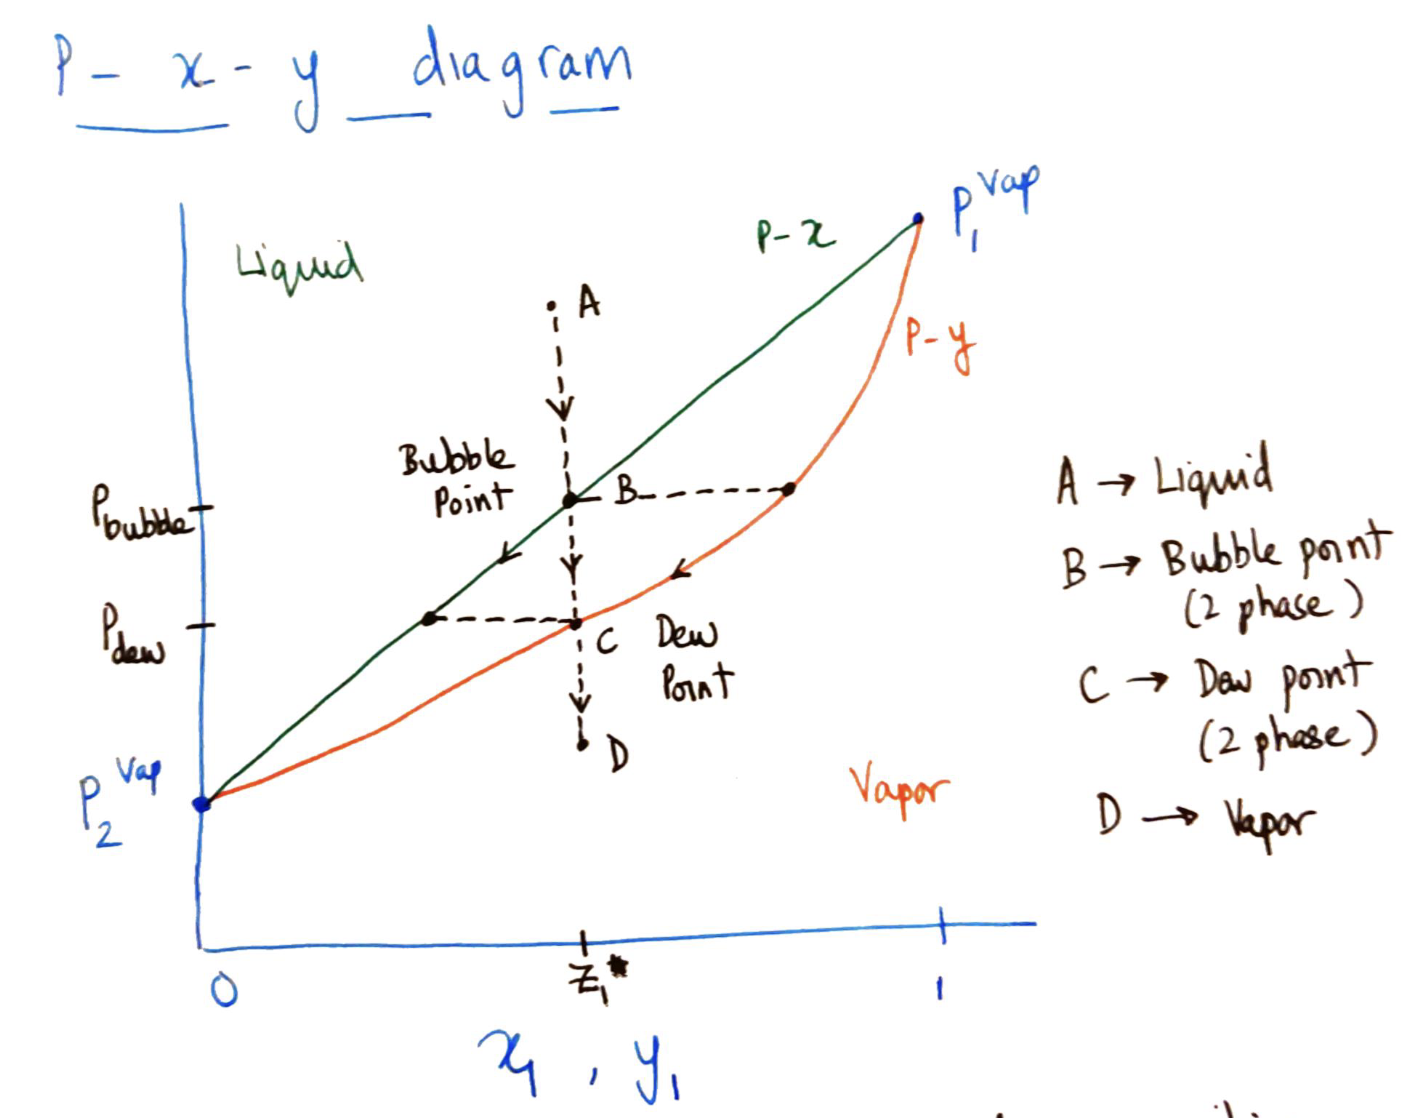
\includegraphics[width=0.52\textwidth, frame]{pxy.png}
    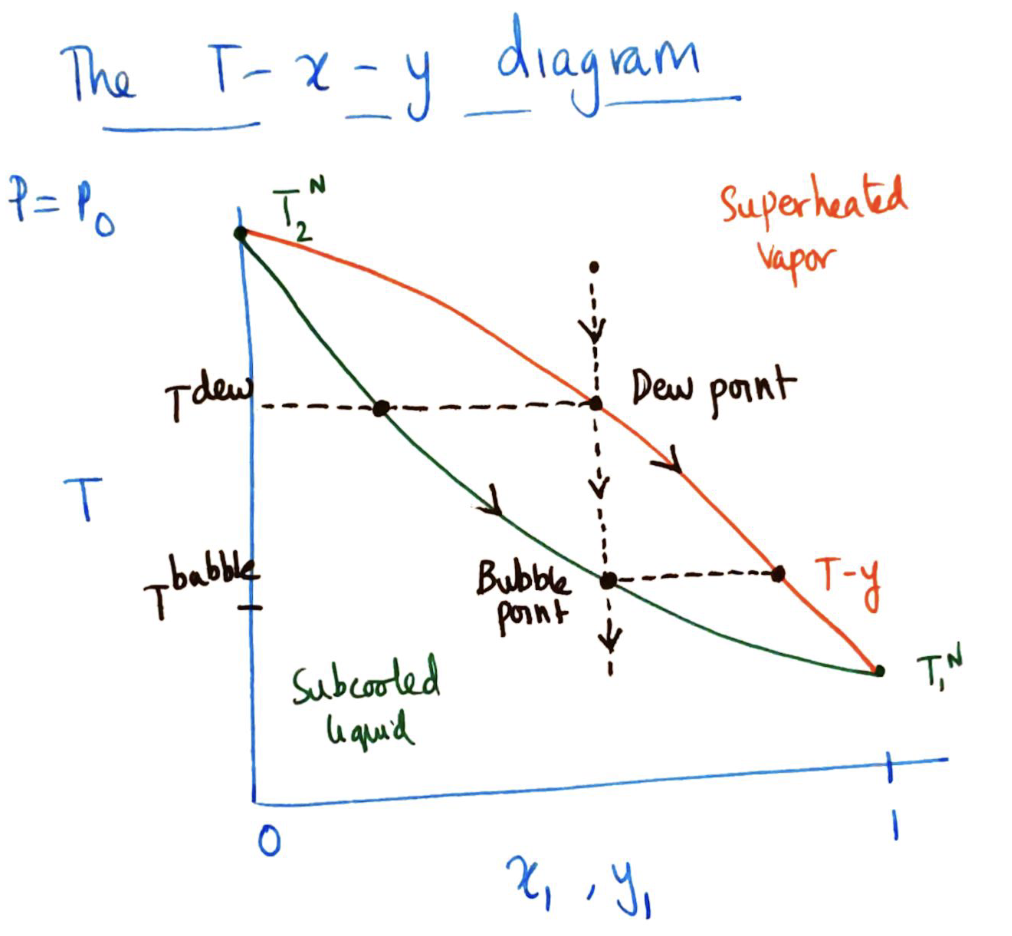
\includegraphics[width=0.442\textwidth, frame]{txy.png}
\end{figure*}
\subsection*{useful vle problem solutions}
bubble pressure
\[\sum x_{i} \gamma_i P^{\text{vap}}_{i}(T) = P_{\text{total}}\]
dew pressure
\[P_{\text{total}} = \frac{1}{\displaystyle\sum \frac{y_{i}}{P^{\text{vap}}_{i}}} = \frac{1}{\displaystyle\sum \frac{y_{i}}{\gamma_i P^{\text{vap}}_{i}}}\]
\[k_i \equiv \frac{y_i}{x_i} = \frac{\gamma_i P^{\text{vap}}_{i} }{P_{\text{total}}} \] 
\[y_{i} = \frac{z_{i} k_{i} }{1 + V(k_{i} -1)} \hspace{2em} x_{i} = \frac{z_{i} }{1 + V(k_{i} -1)}\] 
positive azeotrope
\begin{itemize}
    \item minimum boiling T; maximum pressure
    \item $k_i>1$ before $x_{az}$ (for more volatile)
    \item positive deviation from raoults
\end{itemize}
negative azeotrope
\begin{itemize}
    \item maximum boiling T minimum pressure
    \item $k_i<1$ before $x_{az}$ (for more volatile)
    \item negative deviation from raoults
\end{itemize}
relative volatility
\[\alpha_{12} = \frac{K_1}{K_2} = \frac{\gamma_1 P^\mathrm{vap}_1}{\gamma_2 P^\mathrm{vap}_2}\]
\begin{itemize}
    \item relative volatility = 1 at azeotrope
    \item if pure component limits are on opposite sides of 1, an azeotrope likely exists
\end{itemize}
reflux ratio, $q$
\[q = \frac{L}{D}\]
upper operating line
\[y = \frac{x_{D}}{1+q} + \frac{x_{i}q}{1+q}\]
slope less than 1
lower operating line
\[y = x \left(\frac{ q+\frac{F}{D}}{q+1} \right) - x_{b} \left( \frac{\frac{F}{D} -1}{q+1} \right)\]
slope greater than 1
\subsection*{fugacity of species in mixture}
vapor
\[\bar{f}_{i} = y_{i} P \left( \frac{\bar{f}_{i}}{y_{i}P} \right) = y_i P \left(\frac{f}{P}\right) \]
liquid
\[\bar{f}_{i} = x_{i} \gamma_{i} f_{i}\]

\subsection*{poynting correction}
\begin{align*}
f^{\mathrm{L}}(T,P) &= P^{\mathrm{vap}}(T)
\left(\frac{f}{P}\right)_{\mathrm{sat},T} \exp\!\biggl[\frac{1}{RT}\int_{P^{\mathrm{vap}}(T)}^{P} \underline{V}\,dP\biggr] \\
&= f_{\mathrm{sat}}(T)\exp{\left[{\frac{1}{R T}}\int_{P^{\mathrm{vap}}(T)}^{P}\underline{V}\,d P\right]}
\end{align*}
\subsection*{henry law forms}
\[\bar{f}_{i}^{L} (T,P,\underline{x}) = x_{i} \gamma_{i}^{*}(T,P,\underline{x}) H_{i}(T,P) \tag{molarity} \]
\[ \bar{f}_{i}^{L}(T,P,M_{i}) = M_{i} \gamma_{i}^{\square}(T,P,M_{i})  \mathcal{H} (T,P) \tag{molality} \]
\subsection*{molality henry law}
molality eqn
\[M_{\mathrm{i}}={\frac{n_{\mathrm{i}} \,1000}{m_{\mathrm{s}}n_{\mathrm{s}}}}\]
relating henry coeffs
\[\mathcal{H}_i = \frac{x_{\mathrm{i}}\;1000}{m_{\mathrm{s}}M_{\mathrm{i}}} H_i\]



%%%%%%%%%%%%
% exam 2 
%%%%%%%%%%%%


\twocolumn

\section*{LLE}
\[x_{i}^{I} \gamma_{i}^{I} = x_{i}^{II} \gamma_{i}^{II} \tag{important LLE eqn}\]

\begin{figure}[ht] % Adjusted float specifier to 'ht'
    \centering
    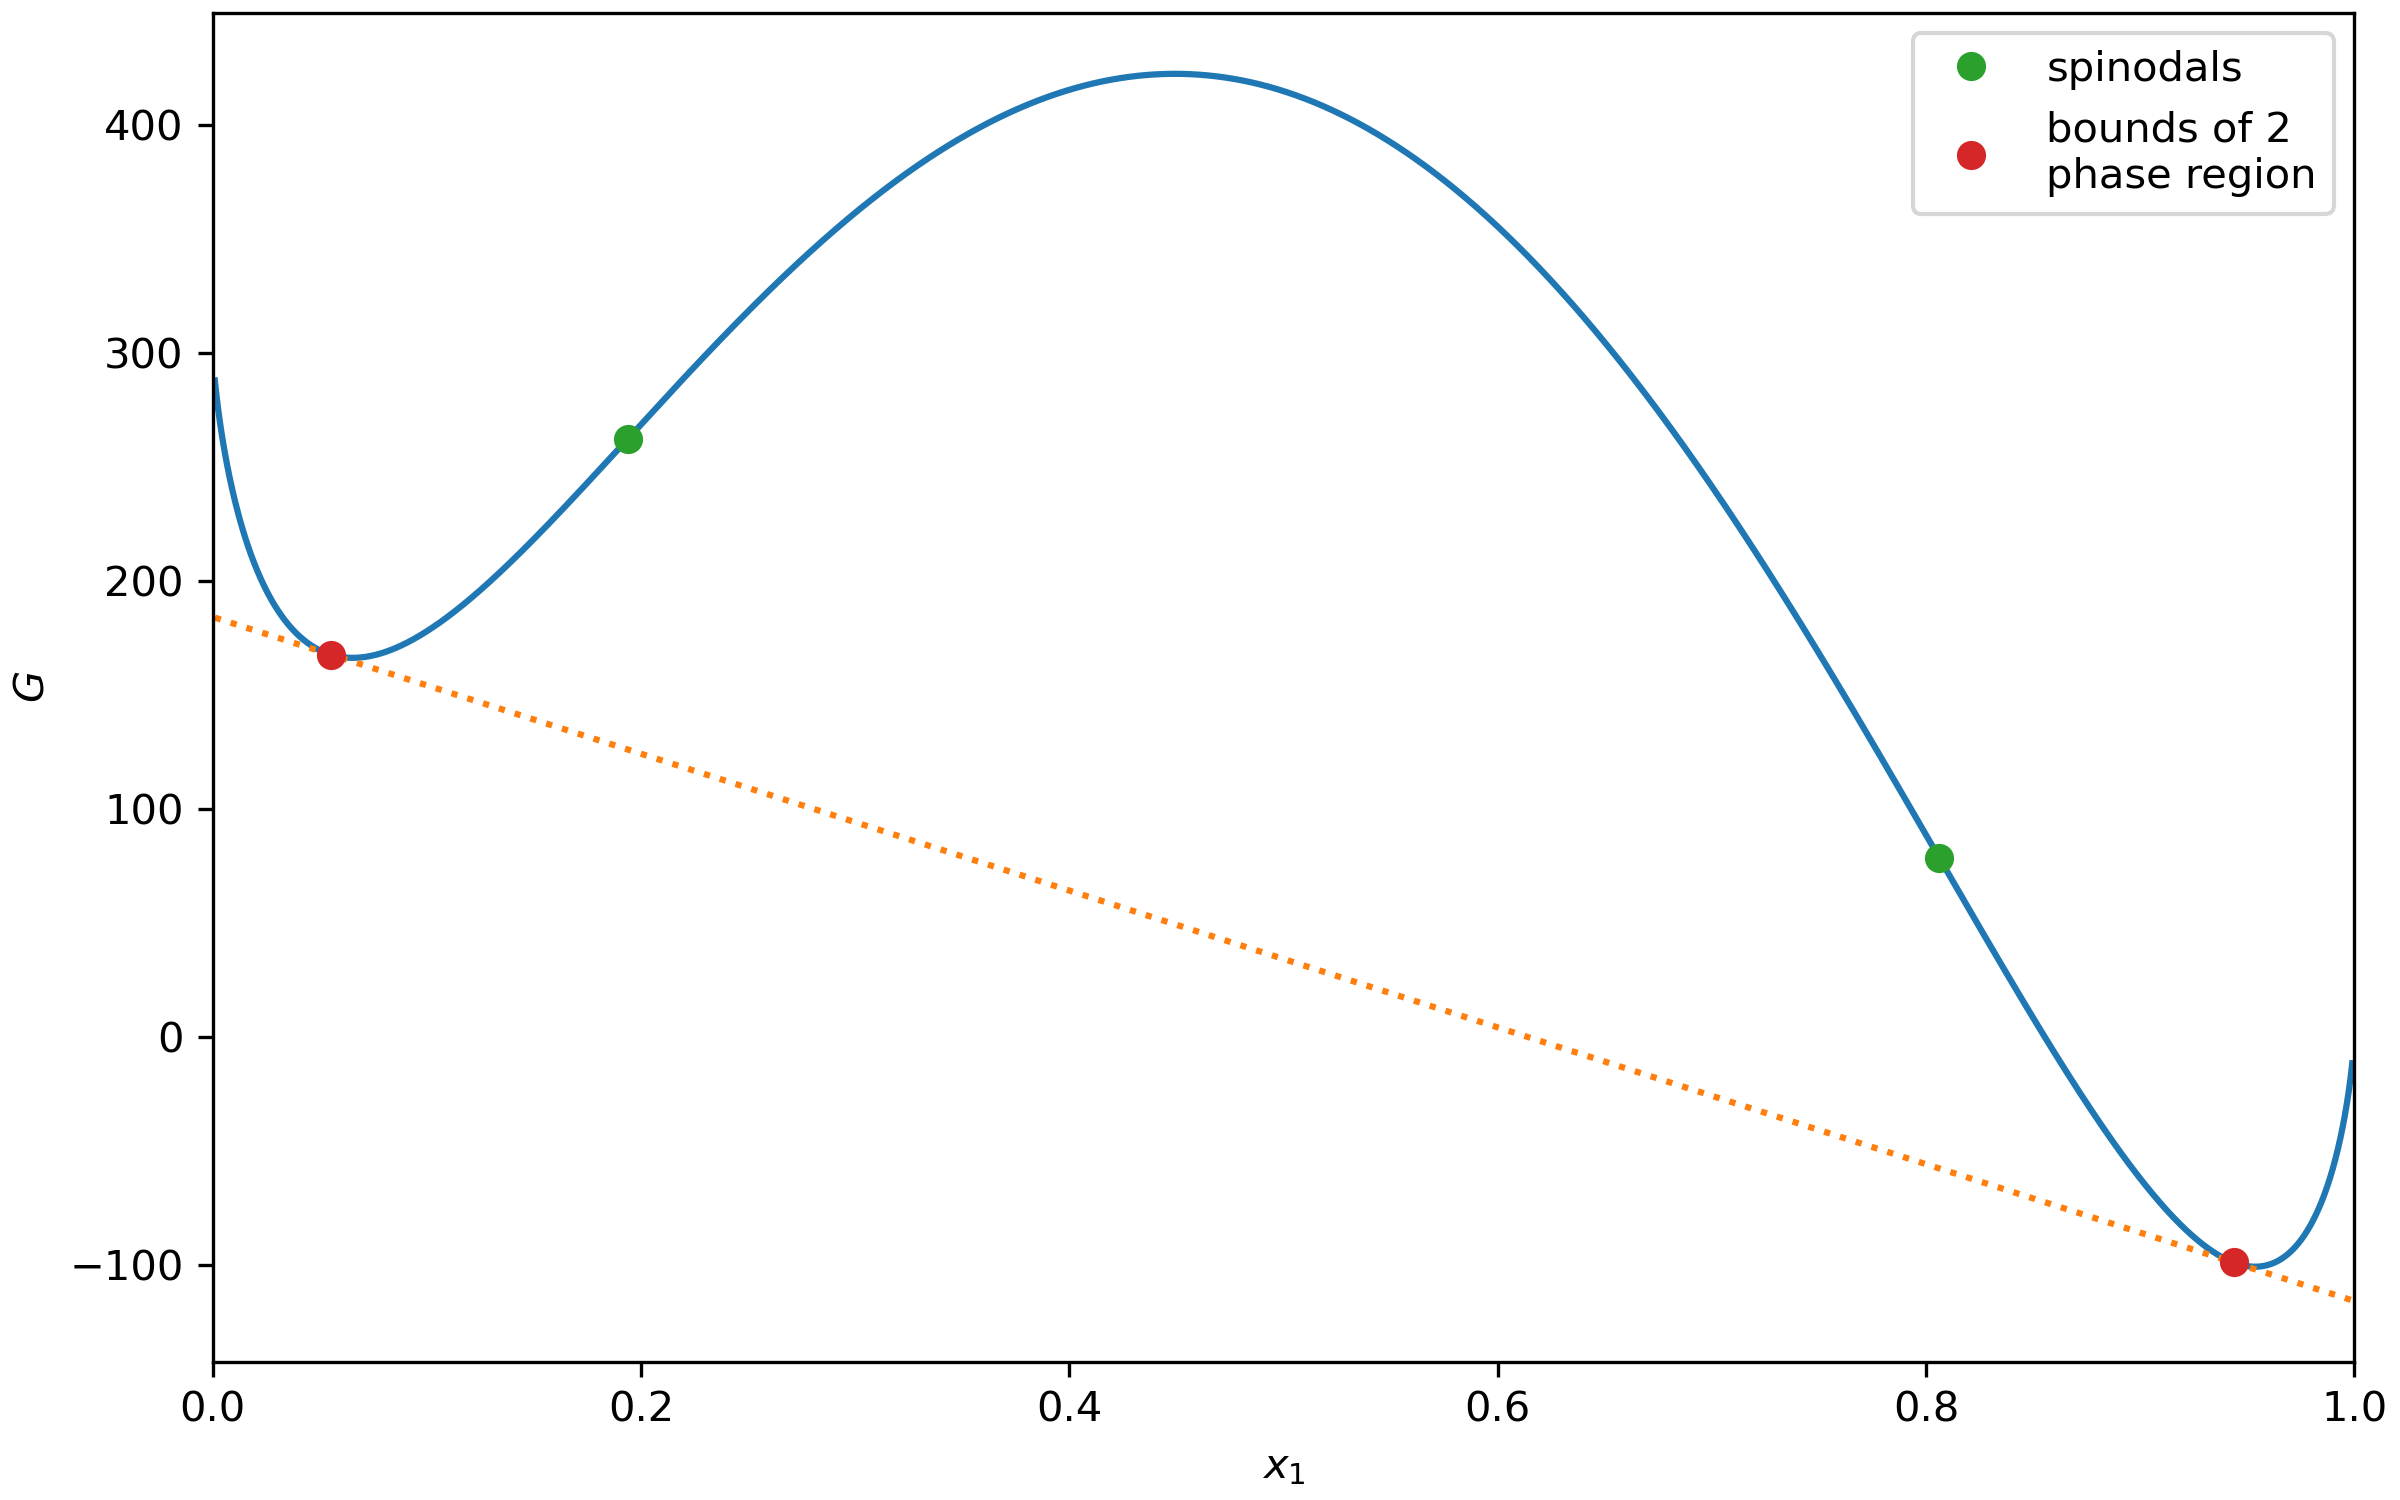
\includegraphics[width=0.48\textwidth, frame]{lle_gibbs.png}
\end{figure}

\begin{itemize}
    \item spinodal points are inflection points
    \item binodals share common tangent line
    \item composition of liquid phases given by binodals
    \item between the bounds and the spinodals is the 'metastable region'
    \item between spinodal points is the region of absolute instability
\end{itemize}
stability criteria
\[ \left(\frac{ \partial^{2} G }{ \partial x^{2} } \right) > 0  \]


\section*{various activity coefficient models}
\subsection*{one constant margules}
\[ \underline{G}^{\mathrm{ex}} = Ax_{1}x_{2} \hspace{3em} \ln \gamma_{1} = \frac{A}{RT}x_{2}^{2} \]
upper consulate temperature
\[ T_\mathrm{uc} = \frac{A}{2R} \]
\subsection*{redlich-kister}
\[ \underline{G}^{\mathrm{ex}} = x_{1}x_{2} (A + B(x_{1}-x_{2}) + C(x_{1}-x_{2})^{2} + \dots) \]
\subsection*{two constant margules}
\[ RT \ln \gamma_{1} = \alpha_{1}x_{2}^{2} + \beta_{1}x_{2}^{3} \]
\begin{itemize}
    \item $\alpha, \beta$ are related to $A,B$ in redlich-kister expansion
\end{itemize}
\subsection*{regular solution}
\begin{itemize}
    \item a regular solution has $\underline{V}^{\mathrm{ex}} = \underline{S}^{\mathrm{ex}} = 0$
\end{itemize}
\[\Phi_{\mathrm{i}}\equiv{\frac{x_{\mathrm{i}}\underline{V}_{\mathrm{i}}}{x_{1}\underline{{{V}}}_{1}+x_{2}\underline{{{V}}}_{2}}} \hspace{3em} \delta_{\mathrm{i}}\equiv\left(\frac{\Delta_{\mathrm{vap}}\underline{U}_{\mathrm{i}}}{V_{\mathrm{i}}}\right)^{1/2}\]
activity coeff
\[\begin{array}{l}{{R T\ \ln\gamma_{1}=\underline{{{V}}}_{1}\Phi_{2}^{2}[\delta_{1}-\delta_{2}]^{2}}}\\ {{R T\ \ln\gamma_{2}=\underline{{{V}}}_{2}\Phi_{1}^{2}[\delta_{1}-\delta_{2}]^{2}}}\end{array}\nonumber\]
\subsection*{van laar model}
\[ \ln \gamma_{1} = \frac{\alpha}{\biggl[  1+ \displaystyle\frac{\alpha x_{1}}{\beta x_{2}} \biggr]^{2}} \hspace{3em} \ln \gamma_{2} = \frac{\beta}{\biggl[  1+ \displaystyle\frac{\beta x_{2}}{\alpha x_{1}} \biggr]^{2}} \]
from infinite dilution
\[
\alpha = \ln \gamma_{1}^{\infty} \quad \quad \beta = \ln \gamma_{2}^{\infty}
\]

from one point
\[\alpha=\left(1+\frac{x_{2}\ln\gamma_{2}}{x_{1}\ln\gamma_{1}}\right)^{2}\ln\gamma_{1}\]
\[\beta=\left(1+\frac{x_{1}\ln\gamma_{1}}{x_{2}\ln\gamma_{2}}\right)^{2}\ln\gamma_{2}\]
from regular solution
\[\alpha=\frac{\underline{V}_{1}}{R T}(\delta_{1}-\delta_{2})^{2} \quad \beta=\frac{\underline{V}_{2}}{R T}(\delta_{1}-\delta_{2})^{2}\]
\begin{itemize}
    \item the $\delta$ are solubility parameters
\end{itemize}
from critical properties
\[\alpha={\frac{b_{1}}{R T}}\left[{\frac{\sqrt{a_{1}}}{b_{1}}}-{\frac{\sqrt{a_{2}}}{b_{2}}}\right]^{2}  \quad \beta={\frac{b_{2}}{R T}}\left[{\frac{\sqrt{a_{1}}}{b_{1}}}-{\frac{\sqrt{a_{2}}}{b_{2}}}\right]^{2}\]
three diff methods for a and b
\[a=\frac{27R^{2}T_{C}^{2}}{64P_{C}}\,\,\mathrm{and}\,\,b=\frac{R T_{C}}{8P_{C}}\]
\[a=3P_{C}\underline{V}_{C}^{2}\ \mathrm{and}\ b=\frac{\underline{V}_{C}}{3}\]
\[a={\frac{9\underline{V}_{C}R T_{C}}{8}}{\mathrm{~and~}}b={\frac{\underline{V}_{C}}{3}}\]
\subsection*{two-parameter wilson model}
\[
\frac{G^{\text{ex}}}{RT} = -x_1 \ln(x_1 + x_2 \Lambda_{12}) - x_2 \ln(x_2 + x_1 \Lambda_{21})
\]
and activity coeffient equations
\[
\ln \gamma_1 = -\ln(x_1 + x_2 \Lambda_{12}) + x_2 \left[ \frac{\Lambda_{12}}{x_1 + x_2 \Lambda_{12}} - \frac{\Lambda_{21}}{x_1 \Lambda_{21} + x_2} \right]
\]
\[
\ln \gamma_2 = -\ln(x_2 + x_1 \Lambda_{21}) - x_1 \left[ \frac{\Lambda_{12}}{x_1 + x_2 \Lambda_{12}} - \frac{\Lambda_{21}}{x_1 \Lambda_{21} + x_2} \right]
\]
\textbf{infinite dilution}
\[
\ln \gamma_1^\infty = -\ln \Lambda_{12} + 1 - \Lambda_{12} 
\]
\[
\ln \gamma_2^\infty = -\ln \Lambda_{21} + 1 - \Lambda_{21}
\]
\begin{itemize}
    \item interestingly the wilson model cannot predict two liquid phases (no solutions to $x_{1}^{I} \gamma_{1}^{I}=x_{1}^{II}\gamma_{1}^{II}$ where $x^{I} \neq x^{II}$)
\end{itemize}

\section*{VLLE}
\[
\mathcal{F} = \mathcal{C} - \mathcal{M} - \mathcal{P} + 2 = 2 - 0 - 3 + 2 = 1
\]
\begin{itemize}
    \item at a given temperature there is only one pressure with VLLE !
    \item higher pressure $\longrightarrow$ two liquids
    \item lower pressure $\longrightarrow$ single liquid and vapor
    \item may be broken into LLE problem for liquid phases for simplicity
\end{itemize}
usually the liquid phases will be nearly pure components so the calculations would be greatly simplified
\[
P_{\mathrm{total}} = P^{\mathrm{vap}}_{1} + P^{\mathrm{vap}}_{2}
\]
\section*{solubility of gas in liquid mixtures}
(letting component 1 be the solute)
\[
x_{1}\gamma_{1}f_{1}^{L} = y_{1} P_{\mathrm{total}}
\]
but this kinda creates an issue since usually the temperature will be above the critical temperature of the solute (think $\mathrm{CO_{2}}$ in water). may use corresponding states to get \(\frac{f^{L}}{P_{c}}\) at \(P=1.013\, \mathrm{bar}\) and then the following correction 
\[
\begin{aligned}
f_{1}^{L}(T,P_{\mathrm{total}}) &= f_{1}^{L}(T,P=1.013\,\mathrm{bar}) \\
&\quad \times \exp\!\left( \frac{\underline{V}_{1}^{L}(P_{\mathrm{total}}-1.013\,\mathrm{bar})}{RT} \right)
\end{aligned}
\]
this is like super gay and annoying, so thankfully there's a simpler way with henry's law coefficients
\[
H_{1}(T,P) = \lim_{ x_{1} \to 0 } \frac{\bar{f}^{L}_{1}}{x_{1}} = \gamma_{1}^{\infty} f^{L}_{1}
\]
which for an ideal application gives this relationship
\[
x_{1}H_{1} = y_{1} P_{\mathrm{total}}
\]
\subsection*{temperature dependence}
\[
\left(\frac{ \partial \ln x }{ \partial T } \right)_{P} \approx -\frac{\Delta_{\mathrm{vap}H}}{RT^{2}}
\]
\begin{itemize}
    \item when \(T<T_{c}\) the enthalpy of vaporization will always be positive
    \item for \(T>T_{c}\) it could be negative, and solubility could increase with temperature
\end{itemize}
\subsection*{solubility of a gas in a salt solution}
we have an empirical relationship for this equilibria
\[
\log \left( \frac{S(M)}{S_{0}} \right) = -k_{s} M
\]
\begin{itemize}
    \item \(k_{s}\) "Satchenow coeff" is specific to every salt and gas pair
    \item \(M\) is the molality of the salt
\end{itemize}
meaning of \(k_{s}\)
\begin{itemize}
    \item positive means gas solubility decreases with salt molality "salting out"
    \item negative k means solubility increases with salt molality "salting in"
    \begin{itemize}
         \item you could add a fuck ton of salt and get the gas "out"
    \end{itemize}
\end{itemize}
\section*{solute partitioning}
\[
K_{x,i}^{I/II} = \frac{x_{i}^{I}}{x_{i}^{II}}
\]
\begin{itemize}
    \item typically subscript gives information about what ratio it relates to (mole fractions or mass fractions or molarities or molalities)
    \item superscript tells you which phase is numerator and which is denominator
\end{itemize}
\subsection*{n-octanol and water}
\begin{itemize}
    \item "amphiphatic" molecule w/ hydrophilic and hydrophobic parts
    \item fairly good model for fatty tissue in animals
\end{itemize}
\[
K_{OW,i} = \frac{C^{O}_{i}}{C^{W}_{i}} = 0.114 \frac{x_{i}^{O}}{x^{W}_{i}}
\]
\begin{itemize}
    \item convention to put organic phase in numerator!
    \item usually very high, so tabulated data is in $\log K_{OW}$
\end{itemize}

\subsection*{solute extraction}
\begin{itemize}
    \item separating based on solubility differences
    \item rinsing toluene with water
\end{itemize}
$q$ is the proportion of solute left after each rinse, $V^{II}$ is the volume of the phase being rinsed, $V^{I}$ is the volume of solvent being used to rinse
\[
q = \frac{V^{II}}{V^{II} + K_{i}V^{I}}
\]
\begin{itemize}
    \item independent of system size
\end{itemize}
if you do $n$ solvent extractions the $q$ at the end is
\[
q_{n} = q^{n}
\]
\begin{itemize}
    \item conclude that more steps = more efficient mixing (on a solvent use basis of what you consider efficiency)
\end{itemize}

\section*{osmotic equilibrium}
two phases separated by a semi-permeable membrane. 
\begin{itemize}
    \item since not all components may go through membrane, the $P^{I}=P^{II}$ equilibrium condition no longer applies
    \item by same reasoning $\bar{f}_{i}^{I}=\bar{f}_{i}^{II}$ only holds for the components which may move, too
\end{itemize}
\[
\pi = P^{II}-P^{I} = \frac{RT}{\underline{V}_{\mathrm{solvent}}} x_{\mathrm{solute}} = \frac{RT}{M_{\mathrm{solute}}}C_{\mathrm{solute}}
\]
\begin{itemize}
    \item only a function of $x_{\mathrm{solute}}$ not of chemistry (colligative properties)
    \item may be used to measure molecular masses for polymers or biomolecules
    \item looks a lot like ideal gas law - only valid for tiny concentrations
\end{itemize}

\subsection*{viral expansion}
\[
\frac{\pi}{RT} = \frac{C_{\mathrm{solute}}}{M_{\mathrm{solute}}} \left[ 1 + B_{2} \left( \frac{C_{\mathrm{solute}}}{M_{\mathrm{solute}}} \right) \dots \right]
\]
\begin{itemize}
    \item a few ways of fitting data to find parameters $B_{2} , M$
    \begin{itemize}
        \item literally no  way this shows up on the exam... but could directly curve fit $\displaystyle\frac{\pi}{RT}$ vs. $C_{\mathrm{solute}}$ for params
    \end{itemize}
\end{itemize}
2nd order polynomial fit version
\[
\frac{\pi}{RT} = \left(\frac{1}{M}\right) C_{s} + \left(\frac{B_2}{M^2}\right) C_{s}^2
\]
linear fit version
\[
\frac{\pi}{RT C_s} = \left(\frac{1}{M}\right) + \left(\frac{B_2}{M^2}\right) C_{s}
\]
what about the units of $B_{2}$ and $M$ (for $R$ and $T$ in SI units). 
\[
B_2 \ [=] \ \frac{\text{m}^3}{\text{mol}} \quad \quad M \ [=] \ \frac{\text{kg}}{\text{mol}}
\]
physical meaning of $B_{2}$?
\begin{itemize}
    \item think about pressure deviating from ideal and what that means for interactions
    \item negative $B_{2}$ indicates favorable interactions by that logic
\end{itemize}

\subsection*{van't hoff factor}
to correct our $\pi$ expression we need to account for different molecules dissolving/dissociating different
\[
i = \frac{\text{apparent  \#  molecules in solution}}{\text{moles of solute dissolved}}
\]
now using this to correct our $\pi$
\[
\pi = i \frac{RTC_{s}}{M_{s}}
\]

\begin{itemize}
    \item now our $\pi$ accounts for salts dissociating while sugars, proteins, polymers don't
\end{itemize}

\section*{Solid Liquid Equilibrium}
of course this starts the same place every equilibrium starts. also daddy sandy treats solids as pure components
\[
f_{i}^{S} = \bar{f}_{i}^{L} = x_{i} \gamma_{i} f_{i}^{L} 
\]
at the melting point
\[
f_{i}^{S}=f_{i}^{L} \longrightarrow 1 = x_{i}^{L} \gamma_{i}^{L}
\]
\begin{itemize}
    \item when not at the melting point it gets a bit harder
\end{itemize}
\[
\begin{aligned}
f_1^L(T, P) &= f_1^S(T, P) \times \exp\biggl[
\frac{1}{RT} \Bigl(
\Delta_{\text{fus}} H(T) \Bigl(1 - \frac{T}{T_m}\Bigr) \\
&\quad + \int_{T_m}^{T} \Delta C_P \, dT 
- T \int_{T_m}^{T} \frac{\Delta C_P}{T} \, dT
\Bigr)
\biggr] \\
\end{aligned}
\]
if we apply this to 1 we get
\[
\begin{aligned}
\ln x_1 \gamma_1 =\; & -\frac{\Delta_{\text{fus}} H(T_m)}{RT} \left[1 - \frac{T}{T_m} \right] \\
                     & - \frac{1}{RT} \int_{T_m}^{T} \Delta C_P \, dT \\
                     & + \frac{1}{R} \int_{T_m}^{T} \frac{\Delta C_P}{T} \, dT
\end{aligned}
\]
if $\Delta C_{p}$ constant
\[
\begin{aligned}
\ln x_1 \gamma_1 =\; & - \frac{\Delta_{\text{fus}} H(T_m)}{RT} \left[ 1 - \frac{T}{T_m} \right] \\[8pt]
                    & - \frac{\Delta C_P}{R} \left[ 1 - \frac{T_m}{T} + \ln\left( \frac{T_m}{T} \right) \right]
\end{aligned}
\]
if $\Delta C_{p}=0$ 
\[
\ln x_1 \gamma_1 = - 
\frac{\Delta_{\text{fus}} H(T_m)}{RT} \left[ 1 - \frac{T}{T_m} \right] 
\]
clausius claperyon equation could be useful
\[
\frac{\Delta_{\text{sub}} H}{RT^2} = \frac{d \ln P^{\text{sub}}}{dT} = \ln (10) \frac{d \log_{10} P^{\text{sub}}}{dT}
\]
different types of points on phase diagram
\begin{itemize}
    \item eutectic: 3 phases present, minimum melting temperature
    \item peritectic: liquid and solid cool and then eventually form a different solid phase
    \item horizontal tie lines
    \item line names (liquidus, solidus)
    \item 2 dof in liquid mixture; 1 dof in any region with tie lines; 0 dof at eutectic
\end{itemize}

\begin{figure}[ht] % Adjusted float specifier to 'ht'
    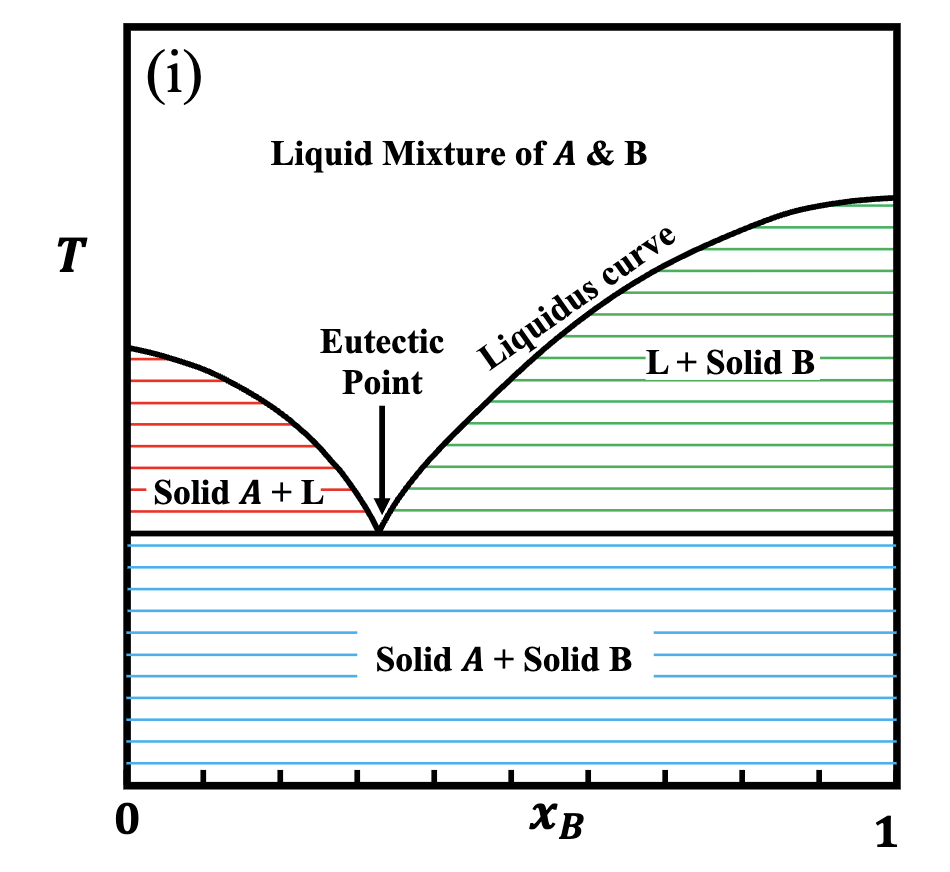
\includegraphics[width=0.442\textwidth, frame]{solids.png}
\end{figure}

\section*{reactions}
stoich coefficients ($\nu$) convention
\begin{itemize}
    \item positive for products
    \item negative for reactants
    \item 0 for bystanders
\end{itemize}
stoich constraint ($A_{i}$ are components)
\[
\sum \nu_{i} A_{i} = 0
\]
equilibrium condition
\[
\sum \nu_{i} \bar{G}_{i} = 0
\]
activity
\[
a = \frac{\bar{f}_{i}}{\bar{f_{i}}^{\circ}}
\]
gibbs compared to standard state
\[
\bar{G}_{i} = \bar{G}_{i}^{\circ}+RT \ln a_{i}
\]
equlibrium constant
\[
K_{a}(T) = \prod a_{i}^{\nu_{i}} = \exp \left(-\frac{\Delta_{\mathrm{rxn}}G^{\circ}}{RT}\right)
\]
relating $\Delta_{\mathrm{rxn}}G$ to formation energies
\[
\Delta_{\mathrm{rxn}}G^{\circ}(T=25^{\circ}\mathrm{C}) = \sum \nu_{i}\Delta_{\mathrm{f}}G_{i}
\]
adjusting $K_{a}$ for different temperatures
\[
\ln\frac{K_{a}(T_{2})}{K_{a}(T_{1})}=\int_{T_{1}}^{T_{2}}\frac{\Delta H_{\mathrm{rxn}}^{\circ}(T)}{R T^{2}}\;d T=-\frac{\Delta_{\mathrm{rxn}}H^{\circ}}{R}\left(\frac{1}{T_{2}}-\frac{1}{T_{1}}\right)
\]
  
\subsection*{different types of systems}
gas phase
\[
{\frac{-\sum\nu_{\mathrm{i}} \underline G_{\mathrm{i}}}{R T}}=\ln\left[\prod_{\mathrm{i}}\left({\frac{y_{\mathrm{i}}({\bar{f}}_{\mathrm{i}}/y_{\mathrm{i}}P)}{(f/P)_{\mathrm{i}}}}\right)^{\nu_{\mathrm{i}}}\right]
\]
ideal gas phase
\[
{\frac{-\sum\nu_{\mathrm{i}} \underline G_{\mathrm{i}}}{R T}}=\ln\left[\prod_{\mathrm{i}}y_{\mathrm{i}}^{\nu_{\mathrm{i}}}\right]
\]
liquid mixture
\[
K_{a}=\prod_{\mathrm{i}}a_{\mathrm{i}}^{\nu_{\mathrm{i}}}=\prod_{\mathrm{i}}(x_{\mathrm{i}}\gamma_{\mathrm{i}})^{\nu_{\mathrm{i}}}=K_{x}K_{\gamma}
\]
ideal liquid mixture
\[
{\frac{-\sum\nu_{\mathrm{i}}\underline{G}_{\mathrm{i}}}{R T}}=\ln\left(\prod_{\mathrm{i}}x_{\mathrm{i}}^{\nu_{\mathrm{i}}}\right)
\]
\subsection*{activities for certain reference states}
species in gaseous mixture
\[
a_{\mathrm{i}}={\frac{y_{\mathrm{i}}P}{1\;\mathrm{bar}}}={\frac{P_{\mathrm{i}}}{1\;\mathrm{bar}}}
\]
liquid mixture; reference of pure liquid
\[
\begin{array}{c}{{a_{\mathrm{i}}=x_{\mathrm{i}}\gamma_{\mathrm{i}}}}\\ {{(\gamma_{\mathrm{i}}\to1\mathrm{~as~}x_{\mathrm{i}}\to1)}}\end{array}
\]
liquid mixture; reference 1 molal soln
\[
\begin{array}{c}{{a_{\mathrm{i}}=M_{\mathrm{i}}\gamma_{\mathrm{i}}^{\square}/(M_{\mathrm{i}}=1)}}\\ {{(\gamma_{\mathrm{i}}^{\square}\to1\mathrm{~as~}M_{\mathrm{i}}\to0)}}\end{array}
\]
liquid mixture; reference is infinite dilution
\[
\begin{array}{l}{{a_{\mathrm{i}}=x_{\mathrm{i}}\gamma_{\mathrm{i}}^{*}}}\\ {{\left(\gamma_{\mathrm{i}}^{*}\longrightarrow1\mathrm{~as~}x_{\mathrm{i}}\rightarrow0\right)}}\end{array}
\]
K based on concentrations
\[
K_{c}=\prod_{\mathrm{\bf{i}}}C_{\mathrm{i}}^{\nu_{\mathrm{i}}}=C^{\sum\nu_{\mathrm{i}}}K_{a}/K_{\gamma}
\]

\subsection*{what reference state to use}
\begin{itemize}
    \item Gas phase 
    \begin{itemize}
        \item Pure component as an ideal gas at reference pressure
    \end{itemize}
    \item Liquid; exists at conditions of mixture
    \begin{itemize}
        \item Pure liquid component at reference pressure
        \item “Liquids that may act as a solvent”
    \end{itemize}
    \item Liquid; does not exist at conditions
    \begin{itemize}
        \item Use Henry law stuffs
    \end{itemize}
\end{itemize}

\section*{ternary systems}
\begin{figure}[ht] % Adjusted float specifier to 'ht'
    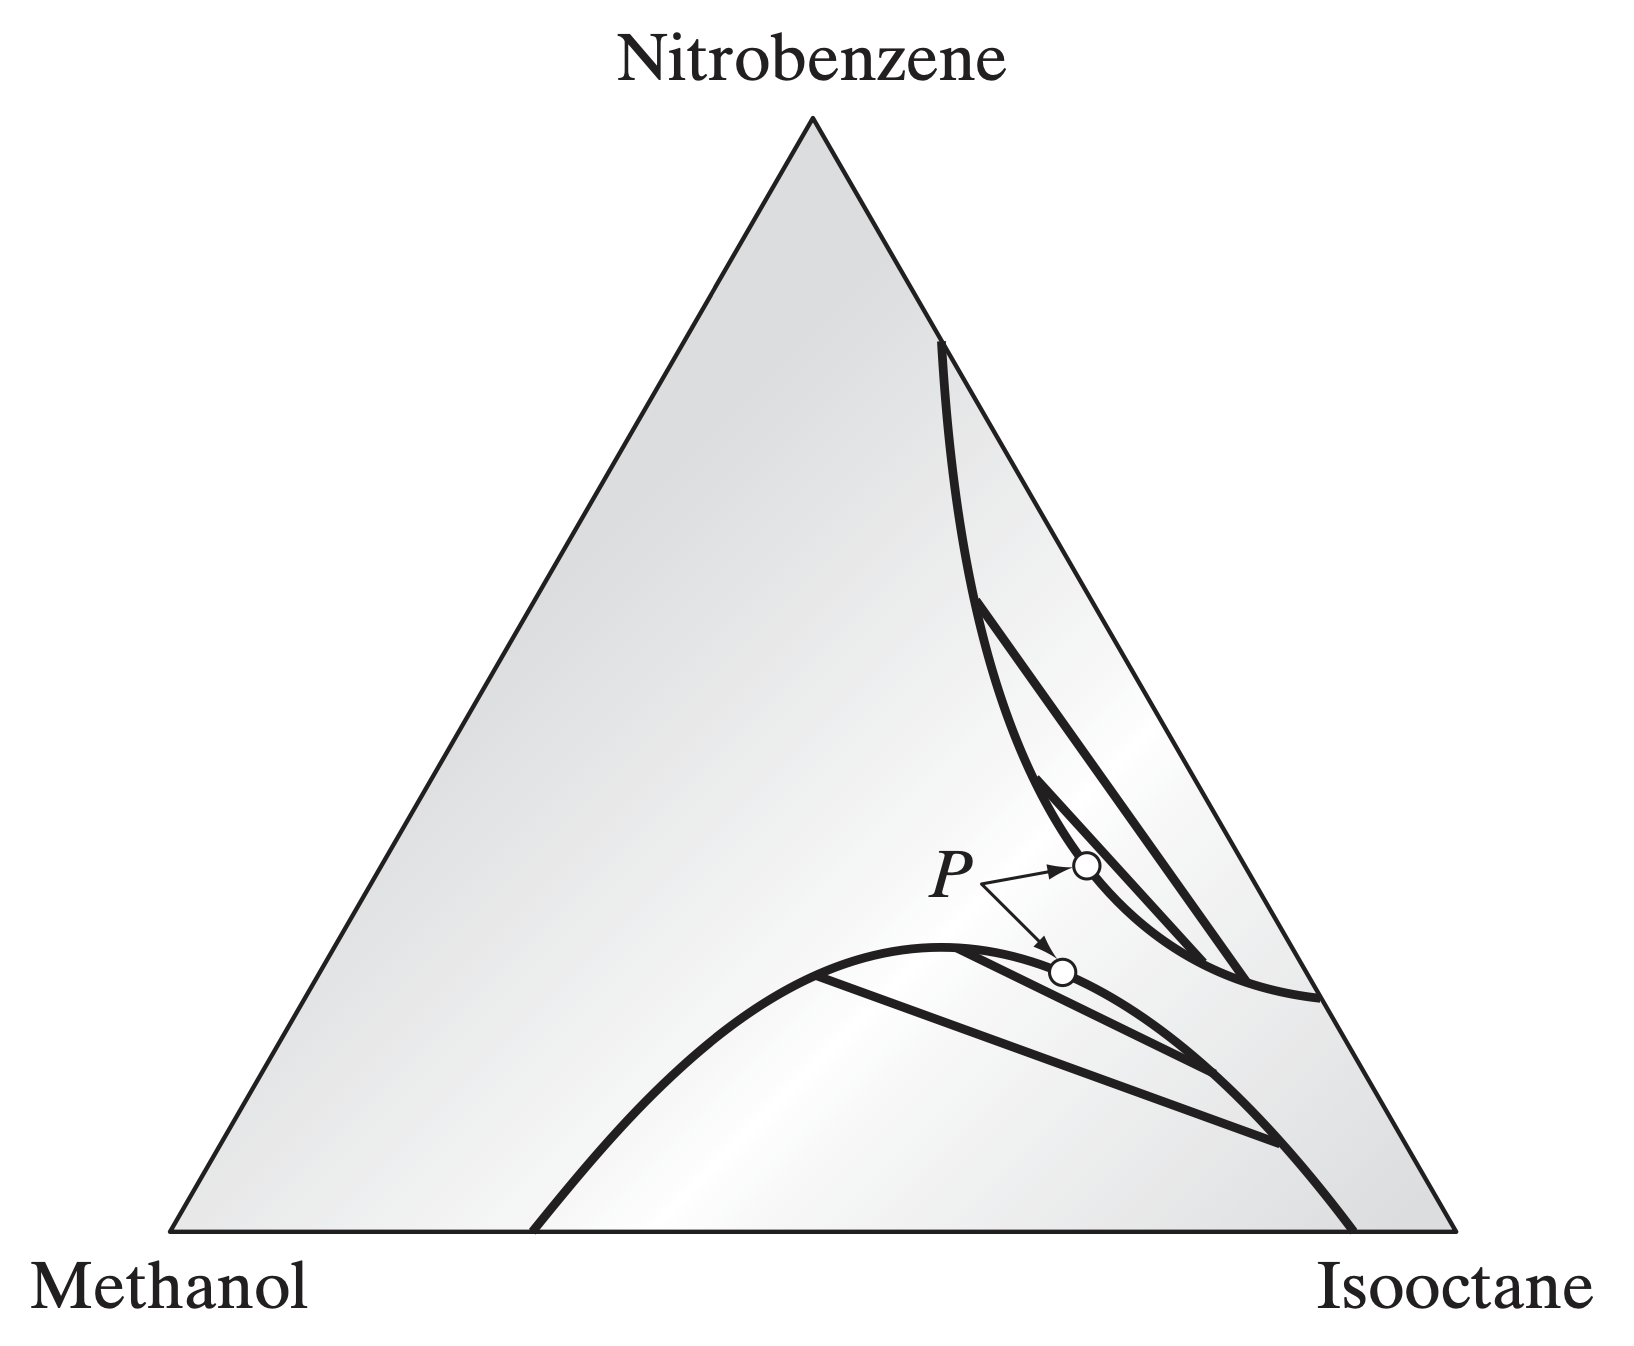
\includegraphics[width=0.442\textwidth, frame]{ternary1.png}
\end{figure}
\begin{figure}[ht] % Adjusted float specifier to 'ht'
    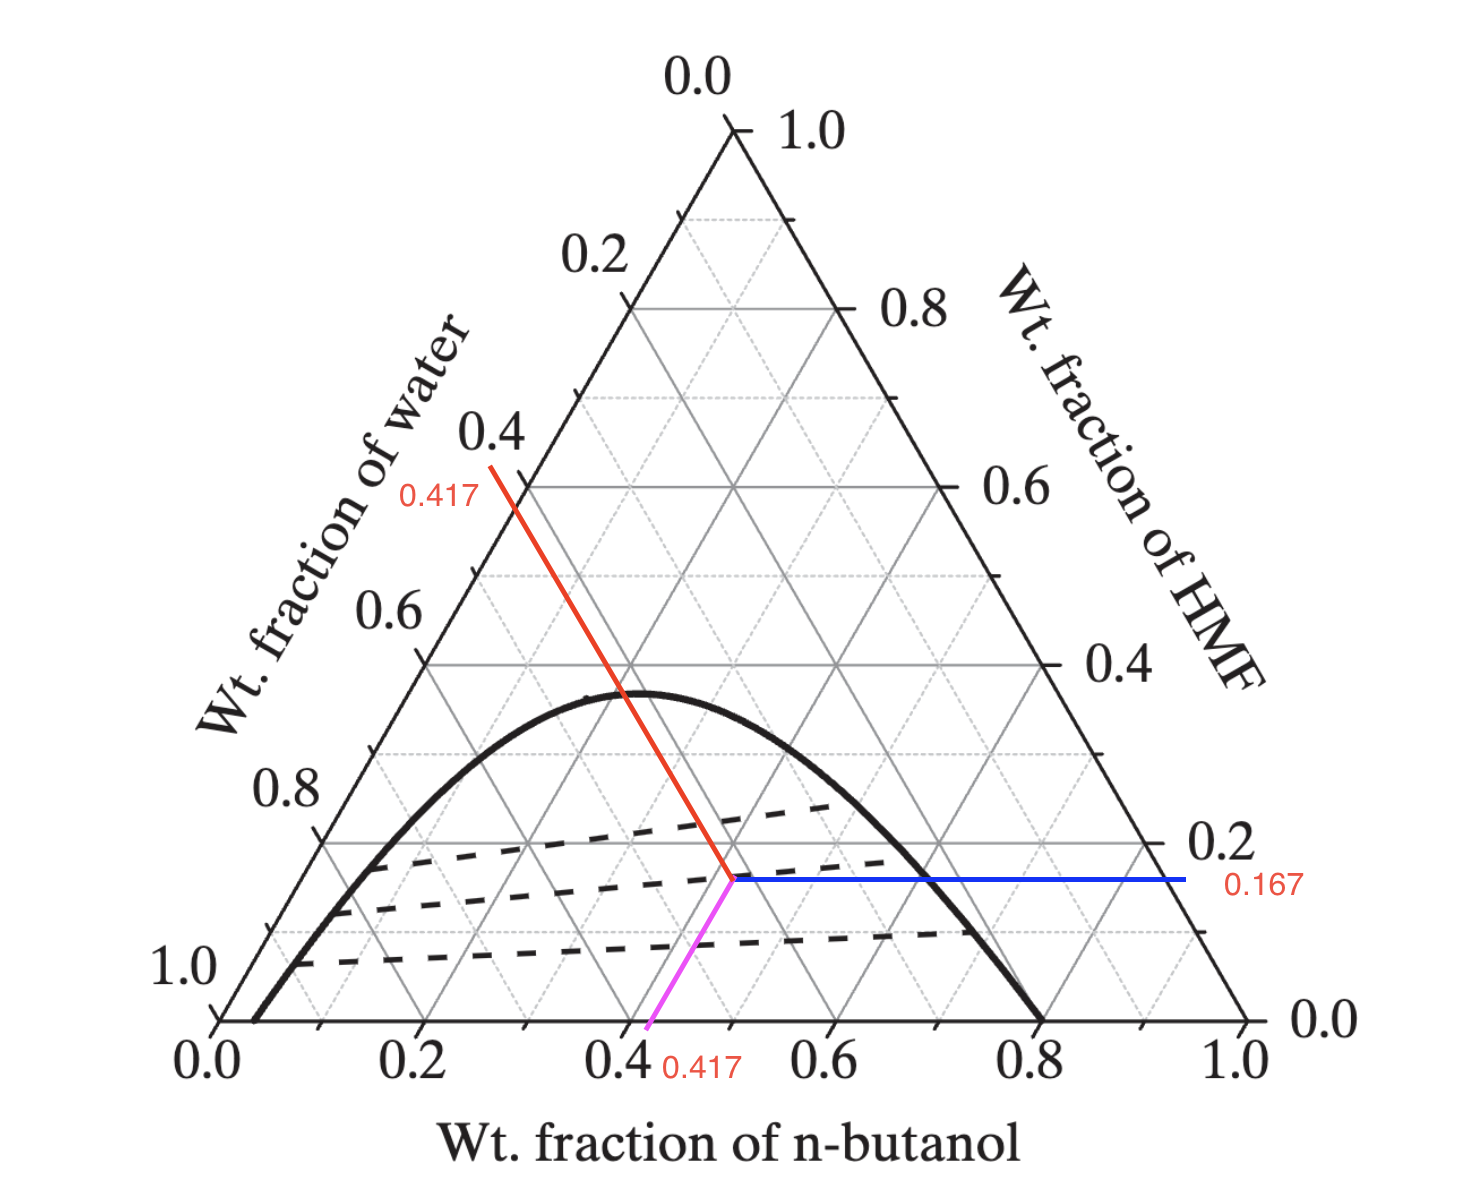
\includegraphics[width=0.442\textwidth, frame]{ternary2.png}
\end{figure}

\begin{figure}[ht] % Adjusted float specifier to 'ht'
    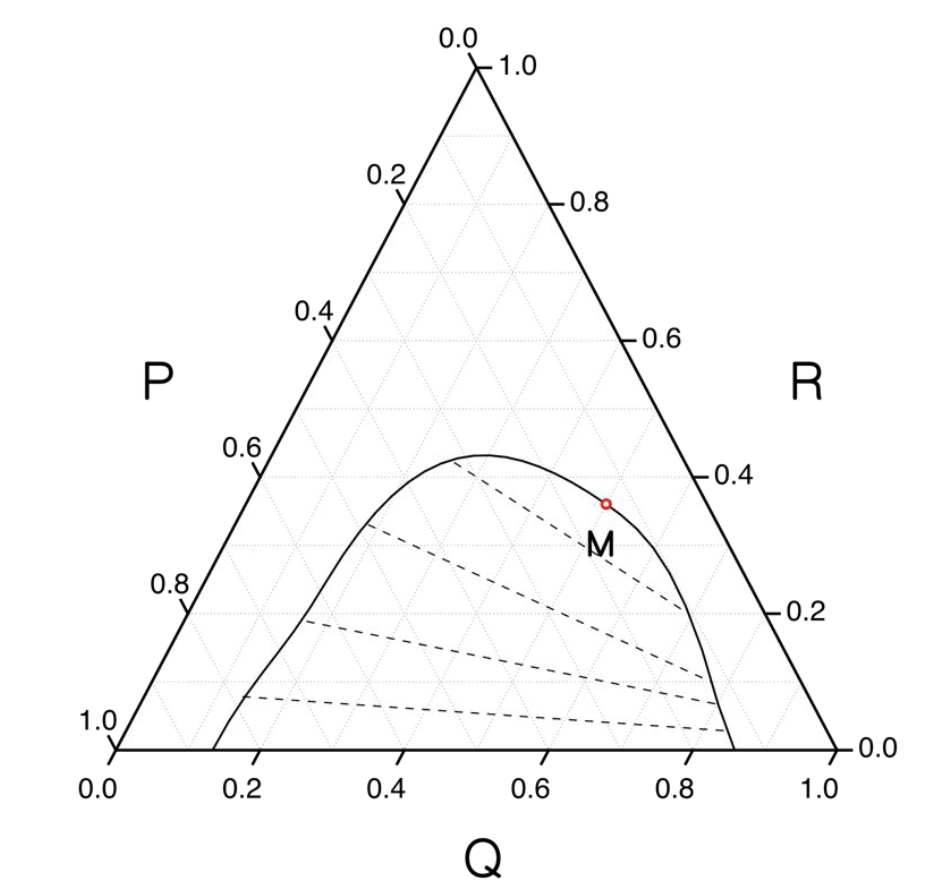
\includegraphics[width=0.442\textwidth, frame]{ternary3.png}
\end{figure}


\end{document}